\documentclass[11pt,titlepage]{amsart}
\usepackage{xcolor}
\usepackage{multicol}
\usepackage{notation}
\usepackage{wrapfig}
\usepackage{multirow}
\usepackage{hyperref}
\usepackage{caption}
\usepackage[anonymous]{atmcs} % for anonymous submission
% \usepackage{atmcs} % for camera-ready
\usepackage{lipsum}
\graphicspath{{C:/Users/story/Projects/team/paper/figures/}}


\begin{document}

\title[]{Topological Equivariant Artist Model}

\author{Hannah~Aizenman}
\address{The Graduate Center, CUNY \\NY, NY, USA}
\email{haizenman@gradcenter.cuny.edu}

\author{Mikael Vejdemo-Johansson}
\address{The Graduate Center, CUNY\\NY, NY, USA}
\email{mvj@math.csi.cuny.edu}


\author{Thomas Caswell}
\address{National Synchrotron Light Source II, Brookhaven National Lab\\ Upton, NY, USA}
\email{tcaswell@bnl.gov}
\author{Michael Grossberg}
\address{The Graduate Center, CUNY\\NY, NY, USA}
\email{mgrossberg@ccny.cuny.edu}

%\keywords{TODO:list keywords}

\begin{abstract}
    The contract data visualization tools make with their users is that a chart is a faithful and accurate visual representation of the numbers it is made from. Motivated by wanting to make better tools, we propose a methodology for fully specifying arbitrary data to visualization mappings in a manner that easily translates to code. We propose that fiber bundles provide a uniform interface for describing a variety of underlying data - tables, images, networks, etc. - in a manner that independently encodes the mathematical structure of the topology and the fields of the dataset. Modeling the data structures that store the datasets as sheaves provide a method for specifying visualization methods that are designed to work regardless of how the dataset is stored - whether the data is on disk, distributed, or on demand. Specifying the visualization library components as natural transforms of sheaves means that the constraints that the component must satisfy to be structure preserving can be specified as the set of morphisms on the data and graphic sheaves, including the structure on the topology and fields of the data.
    Using category theory to formally express how visual elements are constructed means we can translate those expectations into code, which can then be used to enforce the expectation that a visualization tool is faithfully translating between numbers and charts.
\end{abstract}

\maketitle

\section{Intro}
\label{sec:intro}

\begin{wrapfigure}{r}{3.5in}
\begin{center}
    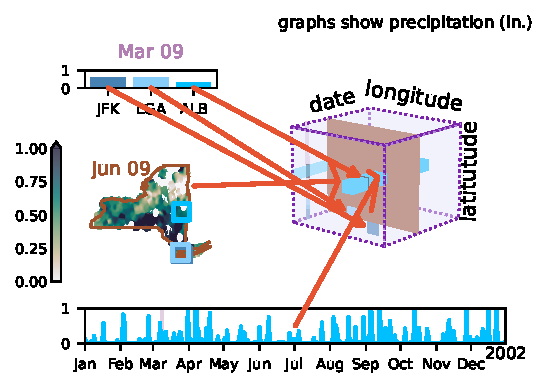
\includegraphics[width=3.5in]{k_different_types.pdf}
\end{center}
\caption{This weather station data has multiple embedded continuities - points at each time and position, timeseries at each position, and maps at each time - that are expected to be homeomorphic to the continuity of their respective visualizations.}
    \label{fig:homeomorphism}
\end{wrapfigure}
Motivated by wanting to make better tools, we propose a methodology for fully specifying arbitrary data to visualization mappings in a manner that easily translates to code. Generally, preserving structure means that a visualization is expected to preserve the $field$ properties and $topology$ of the corresponding dataset, where \textcolor{fiber}{\textbf{field}} is a set of values of the same type and \textcolor{base}{\textbf{topology}} is the connectivity and relative positioning of elements in a dataset \cite{wilkinsonGrammarGraphics2005}.  Field structure is traditionally codified as the Steven's measurement scales \cite{stevensTheoryScalesMeasurement1946}, where each scale is a set of actions on a group Topological structure is generally assumed by visual algorithms \cite{chiTaxonomyVisualizationTechniques2000, toryRethinkingVisualizationHighlevel2004}, but generally do not verify that input structure.
For example, a \texttt{line} algorithm often does not have a way to query whether a list of (x,y) coordinates is the distinct rows, the time series, or the list of stations in \autoref{fig:homeomorphism}. We propose that the bar plot, line plot, and heatmap can be verified as structure preserving because they have a homeomorphic relationship to the 0D ($\bullet$) points, 1D (--) linear, and 2D ($\blacksquare$) surface continuities embedded in the continuous 3 dimensional. Our methodology generalizes Bertin\cite{bertinSemiologyGraphicsDiagrams2011}'s codification of structure,  Mackinlay\cite{mackinlayAutomaticDesignGraphical1987} mathematical formalization, Wilkinson's set theoretic approach \cite{wilkinsonGrammarGraphics2005}, and Kindlemann and Scheidegger's algebraic visualization design (AVD) framework \cite{kindlmannAlgebraicProcessVisualization2014} by explicitly incorporating topology, supporting non-group and non-monoidal structures, and by providing a framework for translating the theoretical ideas into buildable components.



\section{Data Model}
\label{sec:data models}
We extend Butler's proposal of using fiber bundles as an abstraction for visualization data\cite{butlerVectorBundleClassesForm1992,butlerVisualizationModelBased1989} by incorporating Spivak's methodology for encoding named data types from his fiber bundle representation of relational databases \cite{spivakDatabasesAreCategories2010,spivakSimplicialDatabases2009}.


\begin{multicols}{2}
    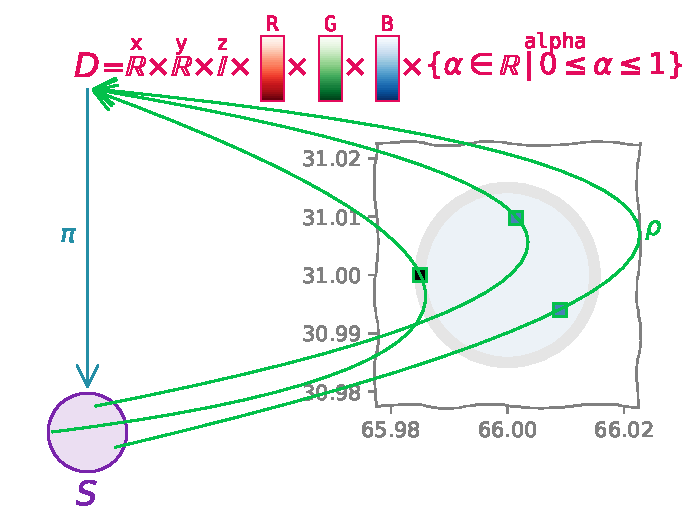
\includegraphics[width=.5\textwidth]{fb_rho.pdf}
    \columnbreak
    \captionof{figure}{The scatter marker is specified by the section $\gsection$, which maps into the fiber $\gfiber$ to retrieve the values that compose into the pixel (approximated as a square) returned by the section function evaluated at each point $\gbasepoint$. The section evaluated over the entire space $\gsection\vert_{S}$ returns the entire scatter mark, shown here in faded form to make it easier to see the individual pixels.}\label{fig:fiber_bundle}

\end{multicols}

\begin{table}[h]
    \begin{tabular}{|r | c c c|}
    \hline
     structure/abstraction & Data & Visual & Graphic\\
    \hline
\textcolor{fiber}{fiber}/\textcolor{total}{total}\ /\textcolor{base}{base} spaces &   \multirow{2}{*}{$\dfiberc \hookrightarrow \dtotalc \xrightarrow{\pi} \dbasec$} &   \multirow{2}{*}{$\vfiberc \hookrightarrow \vtotalc \xrightarrow{\pi} \dbasec$} &  \multirow{2}{*}{$\gfiberc \hookrightarrow \gtotalc \xrightarrow{\pi} \gbasec$}\\
fields/datasets/topology&&&\\
\hline
\textcolor{base}{point}/\textcolor{base}{openset}/\textcolor{base}{base space} &  \multirow{2}{*}{$\dbasepointc \in \opensetc \subseteq \dbasec$} & \multirow{2}{*}{$\dbasepointc \in \opensetc \subseteq \dbasec$} & \multirow{2}{*}{$\gbasepointc \in \opensetgc \subseteq \gbasec$}\\
index/subset/indices & & & \\
\hline
\textcolor{fiber}{fiber space}  record/fields &  $\delementc \in \dfiberc$ & $\velementc \in \vfiberc$ & $\gelementc \in \gfiberc$ \\
\hline
\textcolor{section}{section} dataset & $\cgamma{\dbasec}{\dtotalc} \ni \dsectionc: \dbase \textcolor{section}{\rightarrow} \dfiberc$ & $\cgamma{\dbasec}{\vtotalc} \ni \vsectionc: \dbase \textcolor{section}{\rightarrow} \vfiberc$ &  $\cgamma{\gbasec}{\gtotalc} \ni \gsectionc: \gbase \textcolor{section}{\rightarrow} \gfiberc$ \\
\hline
\textcolor{sheaf}{sheaf} data container  &  \multirow{2}{*}{$\sheafc_{\dbasec, \dtotalc}: \opensetc \rightarrow \cgamma{\opensetc}{\dtotalc\restriction_{\opensetc}}$} &  \multirow{2}{*}{$\sheafc_{\dbasec, \vtotalc}: \opensetc \rightarrow \cgamma{\opensetc}{\vtotalc\restriction_{\opensetc}}$} &   \multirow{2}{*}{$\sheafc_{\gbasec, \gtotalc}: \opensetgc \rightarrow \cgamma{\opensetc}{\gtotalc\restriction_{\opensetgc}}$} \\
&&&\\
        \hline
    \end{tabular}
    \caption{Summary of how the data is abstracted using topological structures}
    \label{tab:data_abstraction}
\end{table}


The indexing space is modeled as a topology $\mathcal{T}$ on the underlying data indexing space because it is a uniform method of describing arbitrary continuity and it provides a method for managing overlapping embedded topologies, such as \autoref{fig:homeomorphism}. Adopting Spivak's fiber bundle construction of types allows our model to reuse types so long as the field names are distinct and encode multi-dimensional fields can be encoded in the same manner as single dimensional fields because domains of types are a mathematical space. We encode data as a \textcolor{section}{section} \dsectionc\ of a bundle because this allows us to incorporate the topology and field types in the data definition $\textcolor{section}{\texttt{dataset}}: \textcolor{base}{\texttt{topology}} \rightarrow \textcolor{fiber}{\texttt{field}}$. Abstracting the data containers as sheaves provides a way of encoding how data containers keep track of the continuity of the data \cite{ghristElementaryAppliedTopology2014} such that visual algorithms developed on this model apply whether the data fits in memory, is distributed, or is streaming.

\section{Artist}
\label{sec:Artist}
We call the mapping from data to graphic $\vartistc:\dsectionc\mapsto\gsectionc$ an \textcolor{artist}{Artist}\footnote{Artists are named for the Artist class in Matplotlib. Artist is the parent class of all the objects that assemble and manage visual elements such as points, lines, and shapes.} and propose that an artist is structure preserving when the artist is implemented as a natural transform on sheaves. This means that the artist satisfies the following constraints, as illustrated in \autoref{fig:artist}:

\begin{multicols}{2}
    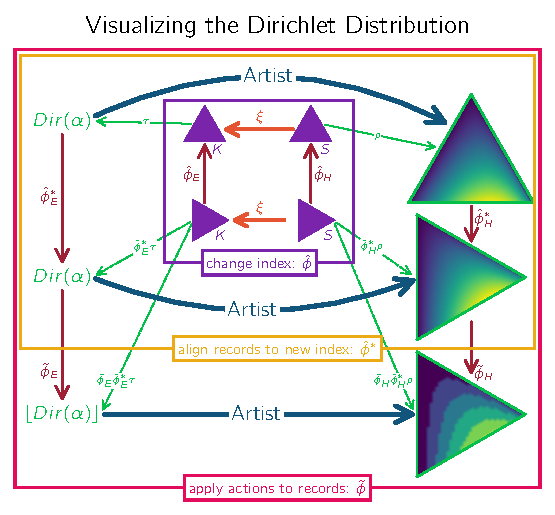
\includegraphics[width=.5\textwidth]{artist_equiv.png}
    \captionof{figure}{}\label{fig:artist}
\columnbreak

\begin{description}
    \item[homeomorphic] there exists a deformation retract $\vindexc: \gbasec\rightarrow\dbasec$ between graphic and artist base space
    \item[topology] the artist is commutative w.r.t. the presheaf morphism $\dfunchc: \dbasepointc^{\prime}\mapsto \dbasepointc$ and pullback $\dfuncpullc \dsectionc \restriction_{\opensetc^{\prime}}: \dsectionc\restriction_{\opensetc^{\prime}} \mapsto \dsectionc \restriction_{\opensetc^{\prime} \circ \dfunchc}$ such that when an index of the record changes the values in the record are unmodified  $\dsectionc(\dbasec) = \dfuncpullc\dsectionc(\dbasepointc^{\prime}) = \dsectionc(\dfunchc(\dbasepointc^{\prime}))$
    \item[fields] the artist is commutative w.r.t. actions on the fiber $\dfunctc \in Hom(\dfiberc, \dfiberc)$, which are the functions between sections $\dfunctc: \dfuncpullc \dsectionc \restriction_{\opensetc^{\prime}} \mapsto \dfuncpullc \dsectionc^{\prime} \restriction_{\opensetc}$. Additionally, $\dfunctc$ must preserve features of $\dfiber$, such as operators, that are defined as part of the structure of $\dfiber$.

\end{description}
\end{multicols}

\begin{figure}[h]
    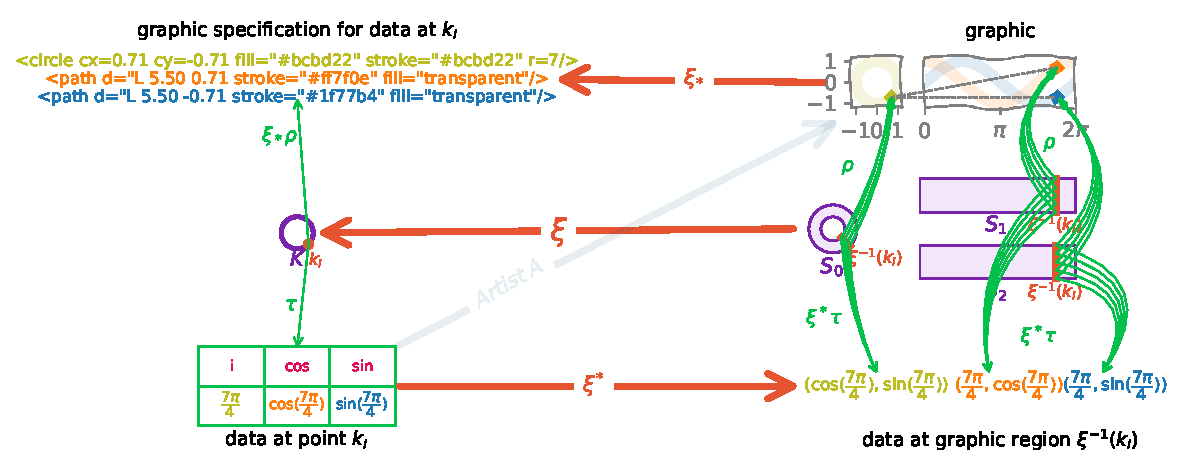
\includegraphics[width=7.16in]{xi_diagram.pdf}
    \caption{The graphics over the orange bands map to the data at the orange point.}
    \label{fig:xi}
\end{figure}
As illustrated in \ref{fig:xi}, the transport functors $(\vindexpush, \vindexpull)$ constructed from $\vindex$ \cite{harder2008lectures} also codify how visual elements correspond to distinct data elements, which is a necessary condition of a visualization being readable\cite{ziemkiewiczEmbeddingInformationVisualization2009}. The pushforward $\vindexpushc$ matches each point in the data space to the specification of the graphic at that point $\vindexpushc\gsectionc(\dbasepointc) = \gsectionc\restriction_{\vindexprec(\dbasepointc)}$, while the pullback $\vindexpull$ matches each point in the graphic space to the data over that point $\vindexpullc\dsectionc(\gbasepointc) = \dsectionc(\vindexc(\gbasepointc)) = \dsectionc(\dbasepointc)$.


\begin{figure*}[h]
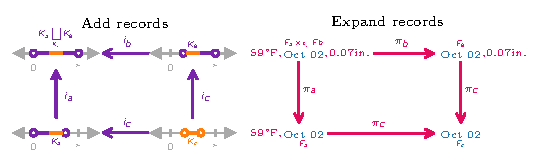
\includegraphics[width=\textwidth]{tex/more_records.png}
\end{figure*}

The topology and fiber categories are equipped with operators to add and extend records, respectively, Since the artist preserves these operators, artists have the property of being composable $\vartistc(\bigsqcup\limits_{i}\dbasec_i, \prod\limits_j\dfiberc_j) = \bigsqcup\limits_i\prod\limits_j\vartistc(\dbasec_i, \dfiberc_j)$


\section{Construction}
The artist can be constructed with an encoding stage $\vchannelc$ and a compositing stage $\vmarkc$ s.t $\vartistc=\vmarkc\circ\vchannelc$. In the \textcolor{artist}{encoding} stage $\vchannelc$, a data bundle is mapped to a visual variable bundle \vchannel, where the fibers of \vchannel\ are an internal library specification. The \textcolor{artist}{compositing} stage $\vmarkc$ is then responsible for assembling  the visual components into a visual element.

\section*{Note}
This is a work in progress, more information can be found at https://github.com/story645/team

\section*{Acknowledgements}
The authors would like to thank the anonymous reviewers who gave constructive feedback on an earlier version of this paper. The authors are also grateful to  the various Matplotlib and Napari contributors, particularly Juan Nunez-Iglesias, and Nicolas Kruchten for their valuable feedback from the library developer perspective. Hannah is also very grateful to Nicolas for the suggestion of augmented notation and to the nlab and wikipedia contributors who wrote clear explanations of many of the topics discussed in this paper. This project has been made possible in part by grant number 2019-207333 (EOSS Cycle 1) and EOSS Cycle 3 Chan Zuckerberg Initiative DAF, an advised fund of Silicon Valley Community Foundation


\bibliographystyle{plain}
\bibliography{references}
\end{document}
